\documentclass[12pt]{article}
\usepackage[T1]{fontenc}
\usepackage[utf8]{inputenc}
\usepackage[polish]{babel}
\usepackage{graphicx}
\usepackage{amsmath}
\usepackage{amssymb}
\usepackage{amsfonts}
\usepackage{float}

\setlength{\textheight}{21cm}

\title{{\bf Zadanie nr 4 -- Modyfikacja algorytmu SABOA\\ zwiększająca różnorodność roju (DESABOA)}\linebreak
Techniki Inteligencji Obliczeniowej w Analizie Danych}
\author{Nikodem Nowak, 251598}
\date{\today}

\begin{document}
\clearpage\maketitle
\thispagestyle{empty}
\newpage
\setcounter{page}{1}

\section{Cel zadania}

Celem zadania było zaproponowanie modyfikacji jednego z rojowych algorytmów
optymalizacji -- GGL-PSOD lub SABOA -- zwiększającej różnorodność roju i poprawiającej
skuteczność metody, a następnie eksperymentalne potwierdzenie jej wyższości nad
algorytmem bazowym. Do modyfikacji wybrano algorytm \textbf{SABOA} (Self-Adaption
Butterfly Optimization Algorithm)~\cite{saboa}, zbudowany na klasycznym algorytmie
\textbf{BOA} (Butterfly Optimization Algorithm)~\cite{boa}. Zaproponowany wariant,
nazwany \textbf{DESABOA} (Diversity-Enhanced SABOA), wprowadza dwa mechanizmy
przeciwdziałające przedwczesnej zbieżności roju.

W ramach zadania zrealizowano:
\begin{itemize}
    \item implementację algorytmu bazowego SABOA oraz proponowanego DESABOA,
    \item dobór parametrów (zakres poszukiwań, wymiar $D$, budżet ewaluacji),
    \item badania na 12 funkcjach z zestawu \textbf{CEC2017} obejmujących wszystkie
          cztery kategorie (unimodalne, multimodalne, hybrydowe, złożone),
    \item uśrednienie wyników po \textbf{51 niezależnych przebiegach} każdej funkcji,
    \item porównanie z SABOA oraz weryfikację istotności statystycznej testem sumy
          rang \textbf{Wilcoxona}.
\end{itemize}

\section{Algorytmy bazowe}

\subsection{BOA}
W algorytmie BOA~\cite{boa} każdy motyl wytwarza zapach o natężeniu zależnym od jakości
rozwiązania, $f = c\cdot I^{a}$, gdzie $I$ to natężenie bodźca (wartość funkcji celu),
$c$ -- modalność sensoryczna, $a$ -- wykładnik. Z prawdopodobieństwem przełączania $p$
motyl wykonuje ruch globalny ku najlepszemu osobnikowi $g^{*}$ lub ruch lokalny względem
dwóch losowych osobników:
\begin{align}
\text{globalny:}\quad & x_i \leftarrow x_i + (r_1 r_2\, g^{*} - x_i)\, f_i,\\
\text{lokalny:}\quad  & x_i \leftarrow x_i + (r_1 r_2\, x_j - x_k)\, f_i,
\end{align}
gdzie $r_1, r_2 \sim U(0,1)$, a $x_j, x_k$ to losowo wybrani osobnicy.

\subsection{SABOA}
SABOA~\cite{saboa} upraszcza BOA, usuwając parametry $c$, $a$ oraz natężenie bodźca $I$.
Jedynym parametrem pozostaje prawdopodobieństwo przełączania $p$. Współczynnik zapachu
jest \emph{samoadaptacyjny} i maleje liniowo w czasie:
\begin{equation}
f = u\left(1 - \frac{t}{T}\right), \qquad u \sim U(0,1),
\end{equation}
gdzie $t$ -- numer iteracji, $T$ -- maksymalna liczba iteracji. Aktualizacja położenia:
\begin{align}
\text{globalny:}\quad & x_i \leftarrow x_i + g^{*} + (x_i - g^{*})\, f,\\
\text{lokalny:}\quad  & x_i \leftarrow 0{,}5\,(g^{*} + w^{*})\, f,
\end{align}
gdzie $w^{*}$ to najgorszy osobnik w populacji. W obu fazach stosowana jest akceptacja
zachłanna (zachowanie nowego położenia tylko gdy poprawia wartość funkcji celu).
Równania przyjęto zgodnie z publiczną implementacją referencyjną, ponieważ artykuł
źródłowy jest płatny.

Mały współczynnik $f\in(0,1)$ oznacza krótkie kroki, przez co rój szybko traci
różnorodność i utyka w minimach lokalnych. To właśnie ta słabość jest celem
zaproponowanej modyfikacji.

\section{Zaproponowana modyfikacja: DESABOA}

DESABOA rozszerza SABOA o dwa mechanizmy zwiększające różnorodność roju.

\subsection{(a) Uczenie przez przeciwności (OBL) w inicjalizacji}
Obok losowej populacji $P=\{x_i\}$ generowana jest populacja przeciwna
\begin{equation}
\breve{x}_{i,j} = lb_j + ub_j - x_{i,j},
\end{equation}
po czym oceniane jest $2N$ punktów i zachowywane $N$ najlepszych. Dzięki temu start
algorytmu jest równomierniej rozłożony w przestrzeni poszukiwań i statystycznie bliższy
optimum~\cite{glpso}.

\subsection{(b) Mutacja sterowana różnorodnością roju}
W każdej iteracji mierzona jest różnorodność roju jako średnia odległość osobników od
centroidu:
\begin{equation}
D_t = \frac{1}{N}\sum_{i=1}^{N}\left\lVert x_i - \bar{x}\right\rVert,
\qquad \bar{x} = \frac{1}{N}\sum_{i=1}^{N} x_i.
\end{equation}
Gdy różnorodność spada poniżej progu, $D_t < \theta\, D_0$ (gdzie $D_0$ to różnorodność
początkowa), lub najlepsze rozwiązanie stagnuje przez ustaloną liczbę iteracji,
$m$ najgorszych osobników jest perturbowanych jednym z dwóch operatorów:
\begin{align}
\text{lot Lévy'ego:}\quad & x_i \leftarrow g^{*} + \alpha\,(ub-lb)\,\mathrm{L\acute{e}vy}(\beta)\odot(x_i - g^{*}),\\
\text{skok Cauchy'ego:}\quad & x_i \leftarrow g^{*} + \gamma\,(ub-lb)\,\mathrm{Cauchy}(0,1),
\end{align}
gdzie krok Lévy'ego wyznaczany jest metodą Mantegny ze wskaźnikiem stabilności $\beta$.
Ciężkie ogony rozkładów Lévy'ego i Cauchy'ego umożliwiają zarówno drobne korekty, jak i
rzadkie duże skoki pozwalające uciec z minimów lokalnych. Re-injekcja przywraca
różnorodność roju, nie niszcząc najlepszych osobników (perturbowani są tylko najgorsi).

\subsection{Schemat działania DESABOA}
\begin{enumerate}
    \item Inicjalizacja populacji z OBL; wyznaczenie $g^{*}$, $w^{*}$, $D_0$.
    \item Dopóki budżet ewaluacji nie został wyczerpany:
    \begin{enumerate}
        \item dla każdego osobnika: faza globalna lub lokalna SABOA (zależnie od $p$),
        \item akceptacja zachłanna, aktualizacja $g^{*}$ i $w^{*}$,
        \item pomiar $D_t$; jeśli $D_t < \theta D_0$ lub stagnacja -- mutacja $m$
              najgorszych osobników lotem Lévy'ego / skokiem Cauchy'ego.
    \end{enumerate}
\end{enumerate}
Wszystkie dodatkowe ewaluacje (OBL, re-injekcja) wliczane są do wspólnego budżetu, więc
porównanie z SABOA pozostaje uczciwe.

\section{Konfiguracja badań}

\begin{table}[H]
\centering
\caption{Parametry eksperymentu.}
\begin{tabular}{|l|c|}
\hline
\textbf{Parametr} & \textbf{Wartość} \\
\hline
Zestaw funkcji & CEC2017 (12 funkcji) \\ \hline
Wymiar $D$ & 10 \\ \hline
Zakres poszukiwań & $[-100, 100]^{D}$ \\ \hline
Liczność populacji $N$ & 30 \\ \hline
Budżet ewaluacji (MAX\_FES) & $10000\cdot D = 100\,000$ \\ \hline
Liczba przebiegów & 51 \\ \hline
Prawd. przełączania $p$ & 0{,}8 \\ \hline
Próg różnorodności $\theta$ & 0{,}10 \\ \hline
Frakcja perturbowanych $m$ & 0{,}20\,$N$ \\ \hline
Lot Lévy'ego $\beta$, $\alpha$ & 1{,}5\,;\ 0{,}01 \\ \hline
Skok Cauchy'ego $\gamma$ & 0{,}10 \\ \hline
\end{tabular}
\end{table}

Funkcje dobrano tak, aby pokryć wszystkie kategorie CEC2017: \textbf{unimodalną} (F1),
\textbf{multimodalne} (F4, F5, F9), \textbf{hybrydowe} (F10, F14, F17) oraz
\textbf{złożone} (F20, F21, F24, F27, F29). Jako miarę jakości przyjęto błąd
$f(x)-f^{*}$, gdzie $f^{*}$ to znane optimum globalne (im niżej, tym lepiej; ideał $=0$).
Liczba iteracji wynika z budżetu ewaluacji, dzięki czemu oba algorytmy zużywają tyle samo
ewaluacji funkcji celu.

\section{Wyniki}

Tabela~\ref{tab:wyniki} zestawia uśrednione wartości błędu. DESABOA uzyskuje niższy błąd
średni na \textbf{każdej} z 12 funkcji, najczęściej o 1--4 rzędy wielkości.

\begin{table}[H]
\centering
\caption{Uśrednione wartości błędu $f(x)-f^*$ po 51 przebiegach (D=10). Niżej = lepiej; wynik lepszy pogrubiono.}
\label{tab:wyniki}
\begin{tabular}{llrr}
\toprule
\textbf{Funkcja} & \textbf{Kategoria} & \textbf{SABOA (śr. $\pm$ odch.)} & \textbf{DESABOA (śr. $\pm$ odch.)} \\
\midrule
F1 & unimodalna & $1.88\cdot10^{10} \pm 6.43\cdot10^{9}$ & $\mathbf{4.86\cdot10^{7} \pm 2.49\cdot10^{7}}$ \\
F4 & multimodalna & $1.99\cdot10^{4} \pm 2.88\cdot10^{3}$ & $\mathbf{1.33\cdot10^{2} \pm 3.29\cdot10^{1}}$ \\
F5 & multimodalna & $1.80\cdot10^{-2} \pm 1.18\cdot10^{-2}$ & $\mathbf{8.08\cdot10^{-5} \pm 1.51\cdot10^{-4}}$ \\
F9 & multimodalna & $2.17\cdot10^{3} \pm 2.76\cdot10^{2}$ & $\mathbf{8.64\cdot10^{2} \pm 2.84\cdot10^{2}}$ \\
F10 & hybrydowa & $1.50\cdot10^{8} \pm 1.71\cdot10^{8}$ & $\mathbf{1.99\cdot10^{4} \pm 1.11\cdot10^{4}}$ \\
F14 & hybrydowa & $6.80\cdot10^{7} \pm 8.96\cdot10^{7}$ & $\mathbf{2.51\cdot10^{5} \pm 2.59\cdot10^{5}}$ \\
F17 & hybrydowa & $1.31\cdot10^{8} \pm 2.25\cdot10^{8}$ & $\mathbf{4.80\cdot10^{4} \pm 2.46\cdot10^{4}}$ \\
F20 & złożona & $1.02\cdot10^{4} \pm 5.82\cdot10^{3}$ & $\mathbf{2.30\cdot10^{2} \pm 7.31\cdot10^{1}}$ \\
F21 & złożona & $2.83\cdot10^{2} \pm 1.77\cdot10^{2}$ & $\mathbf{1.14\cdot10^{2} \pm 1.91}$ \\
F24 & złożona & $1.43\cdot10^{3} \pm 3.22\cdot10^{2}$ & $\mathbf{5.05\cdot10^{2} \pm 2.47\cdot10^{1}}$ \\
F27 & złożona & $9.30\cdot10^{2} \pm 3.84\cdot10^{2}$ & $\mathbf{1.63\cdot10^{2} \pm 1.08\cdot10^{2}}$ \\
F29 & złożona & $4.11\cdot10^{9} \pm 5.12\cdot10^{9}$ & $\mathbf{4.07\cdot10^{6} \pm 6.28\cdot10^{6}}$ \\
\bottomrule
\end{tabular}
\end{table}


\subsection{Krzywe zbieżności}
Rysunki~\ref{fig:conv1}--\ref{fig:conv6} przedstawiają średni błąd (skala logarytmiczna)
w funkcji liczby ewaluacji. SABOA bardzo szybko stagnuje, podczas gdy DESABOA
konsekwentnie obniża błąd dzięki wstrzykiwaniu różnorodności.

\newcommand{\convpair}[3]{%
\begin{figure}[H]
\centering
\includegraphics[width=0.49\textwidth]{figury/convergence_F#1.png}\hfill
\includegraphics[width=0.49\textwidth]{figury/convergence_F#2.png}
\caption{Krzywe zbieżności (CEC2017, D=10).}
\label{fig:conv#3}
\end{figure}}

\convpair{1}{4}{1}
\convpair{5}{9}{2}
\convpair{10}{14}{3}
\convpair{17}{20}{4}
\convpair{21}{24}{5}
\convpair{27}{29}{6}

\subsection{Rozkłady błędu końcowego}
Rysunek~\ref{fig:box} przedstawia rozrzut błędu końcowego (51 przebiegów) dla po jednej
reprezentatywnej funkcji z każdej kategorii.

\begin{figure}[H]
\centering
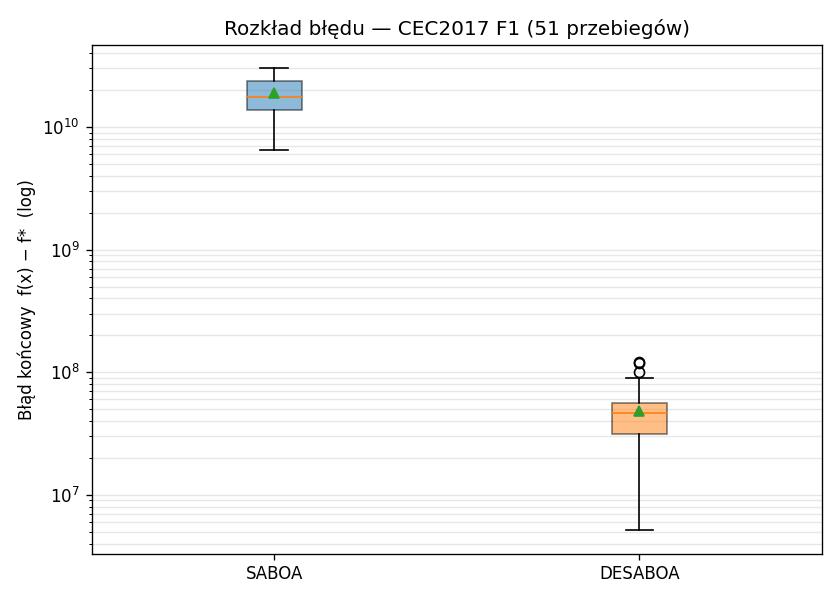
\includegraphics[width=0.49\textwidth]{figury/boxplots_F1.png}\hfill
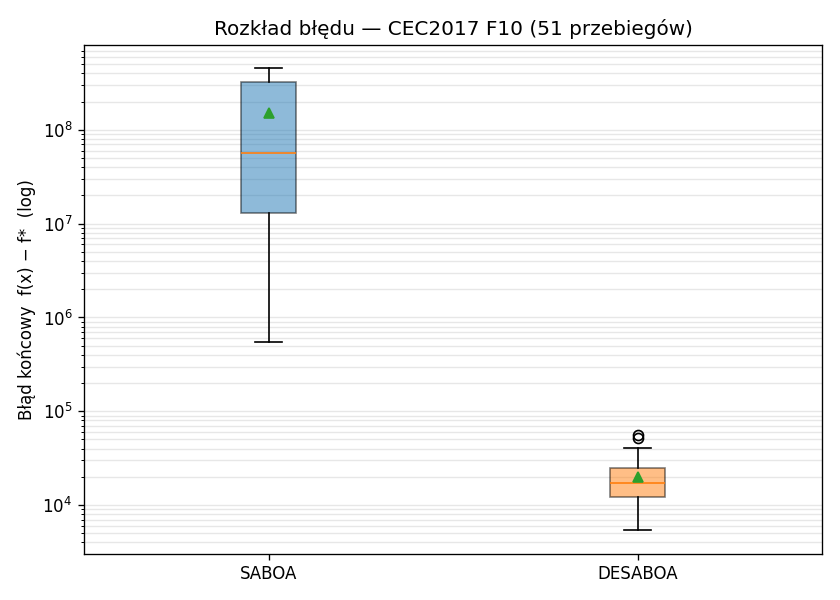
\includegraphics[width=0.49\textwidth]{figury/boxplots_F10.png}\\[2pt]
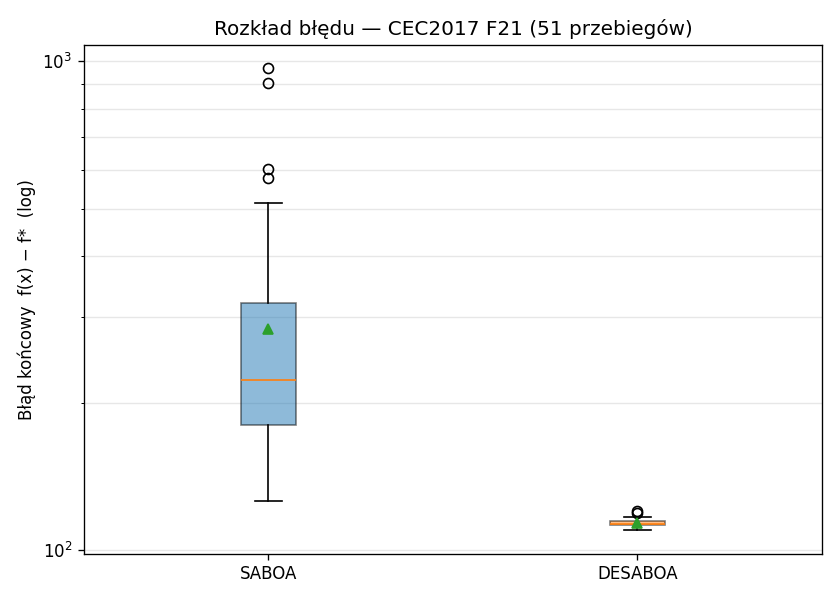
\includegraphics[width=0.49\textwidth]{figury/boxplots_F21.png}\hfill
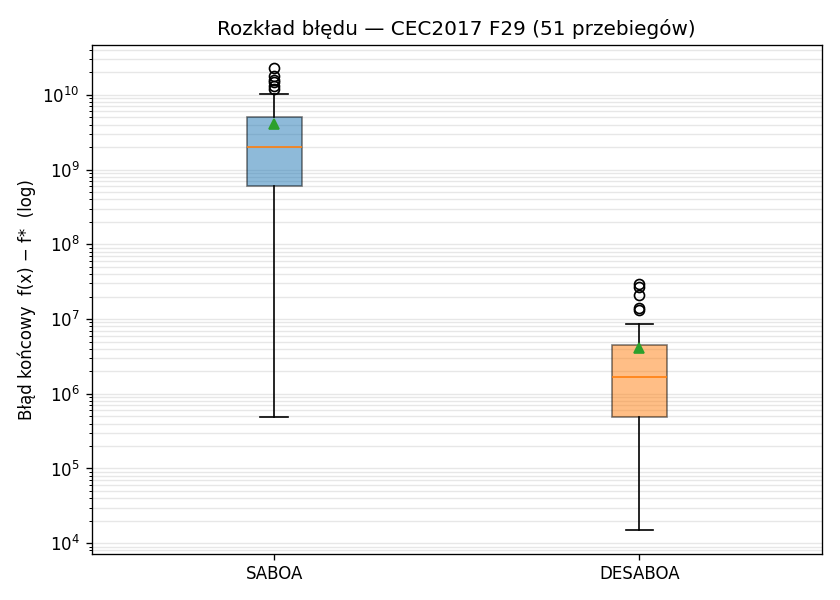
\includegraphics[width=0.49\textwidth]{figury/boxplots_F29.png}
\caption{Rozkłady błędu końcowego: F1 (unimodalna), F10 (hybrydowa),
F21 i F29 (złożone).}
\label{fig:box}
\end{figure}

\section{Test skuteczności (Wilcoxon)}

Wyższość DESABOA zweryfikowano sparowanym testem sumy rang Wilcoxona (dwustronnym,
$\alpha=0{,}05$) na 51 sparowanych przebiegach każdej funkcji. Wyniki zebrano w
tabeli~\ref{tab:wilcoxon}.

\begin{table}[H]
\centering
\caption{Test sumy rang Wilcoxona (sparowany, dwustronny, $\alpha=0{,}05$) dla DESABOA względem SABOA. Zwycięzca wg mediany przy $p<0{,}05$.}
\label{tab:wilcoxon}
\begin{tabular}{|c|c|c|c|c|}
\hline
\textbf{Funkcja} & \textbf{med. SABOA} & \textbf{med. DESABOA} & \textbf{$p$} & \textbf{Zwycięzca} \\
\hline
F1 & $1.74\cdot10^{10}$ & $4.61\cdot10^{7}$ & $5.15\cdot10^{-10}$ & DESABOA \\
\hline
F4 & $2.15\cdot10^{4}$ & $1.25\cdot10^{2}$ & $5.15\cdot10^{-10}$ & DESABOA \\
\hline
F5 & $1.45\cdot10^{-2}$ & $2.32\cdot10^{-5}$ & $5.15\cdot10^{-10}$ & DESABOA \\
\hline
F9 & $2.11\cdot10^{3}$ & $8.51\cdot10^{2}$ & $5.15\cdot10^{-10}$ & DESABOA \\
\hline
F10 & $5.72\cdot10^{7}$ & $1.70\cdot10^{4}$ & $5.15\cdot10^{-10}$ & DESABOA \\
\hline
F14 & $2.14\cdot10^{7}$ & $1.33\cdot10^{5}$ & $5.46\cdot10^{-10}$ & DESABOA \\
\hline
F17 & $3.29\cdot10^{7}$ & $4.39\cdot10^{4}$ & $5.46\cdot10^{-10}$ & DESABOA \\
\hline
F20 & $9.38\cdot10^{3}$ & $2.12\cdot10^{2}$ & $5.15\cdot10^{-10}$ & DESABOA \\
\hline
F21 & $2.23\cdot10^{2}$ & $1.13\cdot10^{2}$ & $5.15\cdot10^{-10}$ & DESABOA \\
\hline
F24 & $1.39\cdot10^{3}$ & $4.95\cdot10^{2}$ & $5.15\cdot10^{-10}$ & DESABOA \\
\hline
F27 & $8.47\cdot10^{2}$ & $1.28\cdot10^{2}$ & $5.15\cdot10^{-10}$ & DESABOA \\
\hline
F29 & $2.02\cdot10^{9}$ & $1.69\cdot10^{6}$ & $5.15\cdot10^{-10}$ & DESABOA \\
\hline
\end{tabular}
\end{table}


Na wszystkich 12 funkcjach różnica jest istotna statystycznie ($p\approx 5\cdot10^{-10}
\ll 0{,}05$), a zwycięzcą zawsze jest DESABOA. Daje to bilans \textbf{12 zwycięstw /
0 remisów / 0 porażek}.

\section{Wnioski}

\begin{itemize}
    \item Zaproponowana modyfikacja DESABOA -- uczenie przez przeciwności oraz mutacja
          sterowana różnorodnością roju -- istotnie poprawia skuteczność SABOA na całym
          badanym zestawie CEC2017.
    \item DESABOA wygrywa \textbf{12/12} funkcji zarówno pod względem błędu średniego,
          jak i istotności statystycznej (test Wilcoxona, $p\approx 5\cdot10^{-10}$).
    \item Największe zyski (do 4 rzędów wielkości) występują na funkcjach hybrydowych i
          złożonych, gdzie bazowy SABOA najszybciej traci różnorodność i przedwcześnie
          zbiega -- co potwierdza, że to właśnie niedobór różnorodności był głównym
          ograniczeniem metody bazowej.
    \item Ponieważ budżet ewaluacji jest identyczny dla obu algorytmów, poprawa wynika
          z lepszej eksploracji przestrzeni, a nie z większej liczby ewaluacji.
\end{itemize}

\begin{thebibliography}{9}
\bibitem{saboa} Y. Fan, J. Shao, G. Sun, X. Shao,
\emph{A Self-Adaption Butterfly Optimization Algorithm for Numerical Optimization
Problems}, IEEE Access, vol. 8, 2020, s. 88026--88041.
\bibitem{boa} S. Arora, S. Singh,
\emph{Butterfly optimization algorithm: a novel approach for global optimization},
Soft Computing, vol. 23, 2019, s. 715--734.
\bibitem{ggl} A. Lin, W. Sun, H. Yu, G. Wu, H. Tang,
\emph{Global genetic learning particle swarm optimization with diversity enhancement
by ring topology}, Swarm and Evolutionary Computation, 2019.
\bibitem{glpso} Y.-J. Gong, J.-J. Li, Y. Zhou, Y. Li, H. S.-H. Chung, Y.-H. Shi, J. Zhang,
\emph{Genetic Learning Particle Swarm Optimization}, IEEE Transactions on Cybernetics,
vol. 46, no. 10, 2016, s. 2277--2290.
\end{thebibliography}

\end{document}
